\documentclass{standalone}
\usepackage{tikz}
\usetikzlibrary{arrows.meta, positioning, calc}

\begin{document}

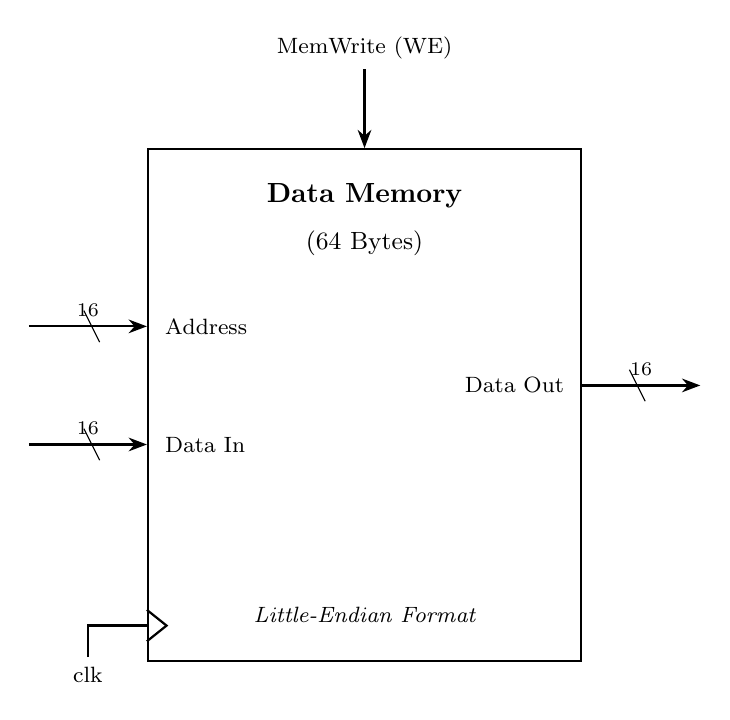
\begin{tikzpicture}[
        box/.style={rectangle, draw, minimum width=5.5cm, minimum height=6.5cm, thick, fill=white},
        port/.style={font=\footnotesize},
        label/.style={font=\scriptsize},
        arrow/.style={->, >=Stealth, thick}
    ]
    
    % Main Box
    \node[box] (mem) at (0,0) {};
    
    % Header Section
    \node[font=\bfseries, yshift=-0.6cm] (title) at (mem.north) {Data Memory};
    \node[font=\small, below=0.05cm of title] {(64 Bytes)};
    
    % Footer Section
    \node[font=\itshape\footnotesize, yshift=0.6cm] at (mem.south) {Little-Endian Format};
    
    % --- Left Side Inputs ---
    
    % Address Input
    \draw [arrow] ($(mem.west)+(-1.5, 1.0)$) -- ($(mem.west)+(0, 1.0)$)
    node[midway, above, label] {16}
    node[pos=1, anchor=west, port, xshift=0.1cm] {Address};
    \draw ($(mem.west)+(-0.8, 1.2)$) -- ($(mem.west)+(-0.6, 0.8)$);
    
    % Data In Input
    \draw [arrow] ($(mem.west)+(-1.5, -0.5)$) -- ($(mem.west)+(0, -0.5)$)
    node[midway, above, label] {16}
    node[pos=1, anchor=west, port, xshift=0.1cm] {Data In};
    \draw ($(mem.west)+(-0.8, -0.3)$) -- ($(mem.west)+(-0.6, -0.7)$);
    
    % --- Right Side Output ---
    
    % Data Out Output
    \draw [arrow] ($(mem.east)+(0, 0.25)$) -- ($(mem.east)+(1.5, 0.25)$)
    node[midway, above, label] {16}
    node[pos=0, anchor=east, port, xshift=-0.1cm] {Data Out};
    \draw ($(mem.east)+(0.6, 0.45)$) -- ($(mem.east)+(0.8, 0.05)$);
    
    % --- Top Control ---
    
    % Write Enable (MemWrite)
    \draw [arrow] ($(mem.north)+(0, 1)$) -- (mem.north)
    node[pos=0, above, port] {MemWrite (WE)};
    
    % --- Clock with shortened horizontal line and lowered triangle ---
    
    % Target point lowered from -2.2 to -2.8
    \coordinate (clk_target) at ($(mem.west)+(0, -2.8)$);
    
    % Draw line: Vertical start remains 0.75cm away
    \draw [thick] ($(mem.west)+(-0.75, -3.2)$) node[below, port] {clk}
    |- (clk_target);
    
    % The Triangle
    \draw [thick] ($(clk_target)+(0, 0.2)$) -- ++(0.25, -0.2) -- ++(-0.25, -0.2);
    
\end{tikzpicture}

\end{document}